\documentclass[12pt, openany, letterpaper]{memoir}
\usepackage{HomeworkStyle}

\begin{document}

\begin{center}
	{\large Homework 4 -- Physical Transformations of Pure Substances}
\end{center}

Name: \rule[-.1mm]{15em}{0.1pt}

\begin{description}
	\item [Exercise 4A.1(a)] ~ (5 points)

	      How many phases are present at each of the points marked in Fig. 4.1a?

	      \noindent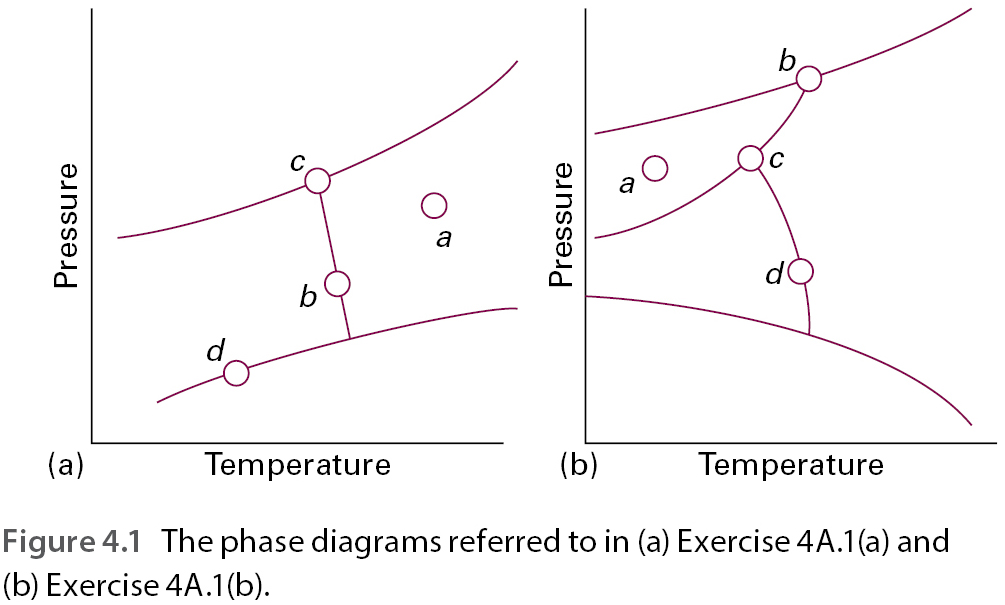
\includegraphics[width=0.5\linewidth]{Phase_Diagrams}
	\item [Exercise 4A.3(a)] ~ (5 points)

	      What is the maximum number of phases that can be in mutual equilibrium in a two-component system?

	      \vspace{10em}
	\item [Exercise 4B.6(a)] ~ (5 points)

	      The vapour pressure of dichloromethane at $24.1^\circ C$ is $53.3~kPa$ and its enthalpy of vaporization is $28.7~\nicefrac{kJ}{mol}$. Estimate the temperature at which its vapour pressure is $70.0~kPa$.



	      \vspace{10em}
	\item [Exercise 4B.8(a)] ~ (10 points)

	      The vapour pressure of benzene between $10^\circ C$ and $30^\circ C$ fits the expression:

	      $\log_{10}~\nicefrac{p}{torr} = 7.960-\dfrac{\nicefrac{1780}{K}}{T}$

	      Calculate (i) the enthalpy of vaporization and (ii) the normal boiling pont of benzene.

	      \vspace{20em}
	\item [Exercise 4B.9(a)] ~ (5 points)

	      When benzene freezes at $1.00~atm$ and $5.5^\circ C$ its density changes from $0.879~\nicefrac{g}{cm^3}$ to $0.891~\nicefrac{g}{cm^3}$. Its enthalpy of fusion is $10.59~\nicefrac{kJ}{mol}$. Estimate the freezing point of benzene at $1000.0~atm$.

	      \vspace{15em}
\end{description}

\newpage
\pagestyle{empty}
\addtocounter{page}{-1}
\newgeometry{margin=1.25in}
\section*{\emph{A Litany for Survival}}
\paragraph{By Audre Lorde}~

\vspace{1em}\noindent
\begin{minipage}[t]{0.56\linewidth}
	For those of us who live at the shoreline\\
	standing upon the constant edges of decision\\
	crucial and alone\\
	for those of us who cannot indulge\\
	the passing dreams of choice\\
	who love in doorways coming and going\\
	in the hours between dawns\\
	looking inward and outward\\
	at once before and after\\
	seeking a now that can breed\\
	futures\\
	like bread in our children’s mouths\\
	so their dreams will not reflect\\
	the death of ours;

	For those of us\\
	who were imprinted with fear\\
	like a faint line in the center of our foreheads\\
	learning to be afraid with our mother’s milk\\
	for by this weapon\\
	this illusion of some safety to be found\\
	the heavy-footed hoped to silence us\\
	For all of us\\
	this instant and this triumph\\
	We were never meant to survive.
\end{minipage}
\begin{minipage}[t]{0.45\linewidth}
	And when the sun rises we are afraid\\
	it might not remain\\
	when the sun sets we are afraid\\
	it might not rise in the morning\\
	when our stomachs are full we are afraid\\
	of indigestion\\
	when our stomachs are empty we are afraid\\
	we may never eat again\\
	when we are loved we are afraid\\
	love will vanish\\
	when we are alone we are afraid\\
	love will never return\\
	and when we speak we are afraid\\
	our words will not be heard\\
	nor welcomed\\
	but when we are silent\\
	we are still afraid

	So it is better to speak\\
	remembering\\
	we were never meant to survive.
\end{minipage}
\end{document}
